\documentclass{beamer}
\usetheme{Warsaw} % Temas
\usecolortheme{crane} % Cores do tema
\usecolortheme{beaver} % Cores do tema
\usepackage[brazil]{babel} 
\usepackage{lmodern}
\usepackage[utf8]{inputenc}	
\usepackage{amsmath}
\usepackage{color}
\usepackage{graphicx}
\usepackage{microtype}
\usepackage{amsmath}
\usepackage{amssymb,url}
\usepackage{xcolor, tikz,bm,colortbl}
\usepackage[br]{nicealgo}
\usepackage{ragged2e}
\definecolor{Scarlet}{RGB}{140,17,17}
\definecolor{darkgreen}{RGB}{0, 94, 11}
\setbeamertemplate{caption}[numbered]

\usepackage[backend=bibtex, style=footnote-dw]{biblatex}
\bibliography{references}

\begin{document}
\title[Título pequeno para os slides]
{Título Principal}  
\author{Autor}
\institute{Faculdade de Ciências (FC) - Campus Bauru \\ Universidade Estadual Paulista ``Júlio de Mesquita Filho''}
\date{\textbf{Orientador:} Prof. Dr. \\~\\ Tipo de Apresentação \\ \today \\ \hspace*{9.8cm} 
\includegraphics[height=0.5cm]{figs/unesp-logo.png}} 

\begin{frame}
\titlepage
\end{frame}

\begin{frame}\frametitle{Sumário}\footnotesize \tableofcontents
\end{frame} 

\section{Seção 1} 
\subsection{Utilizando Figuras}
\begin{frame}\frametitle{Utilizando Figuras} 
\begin{figure}[h]
\centering
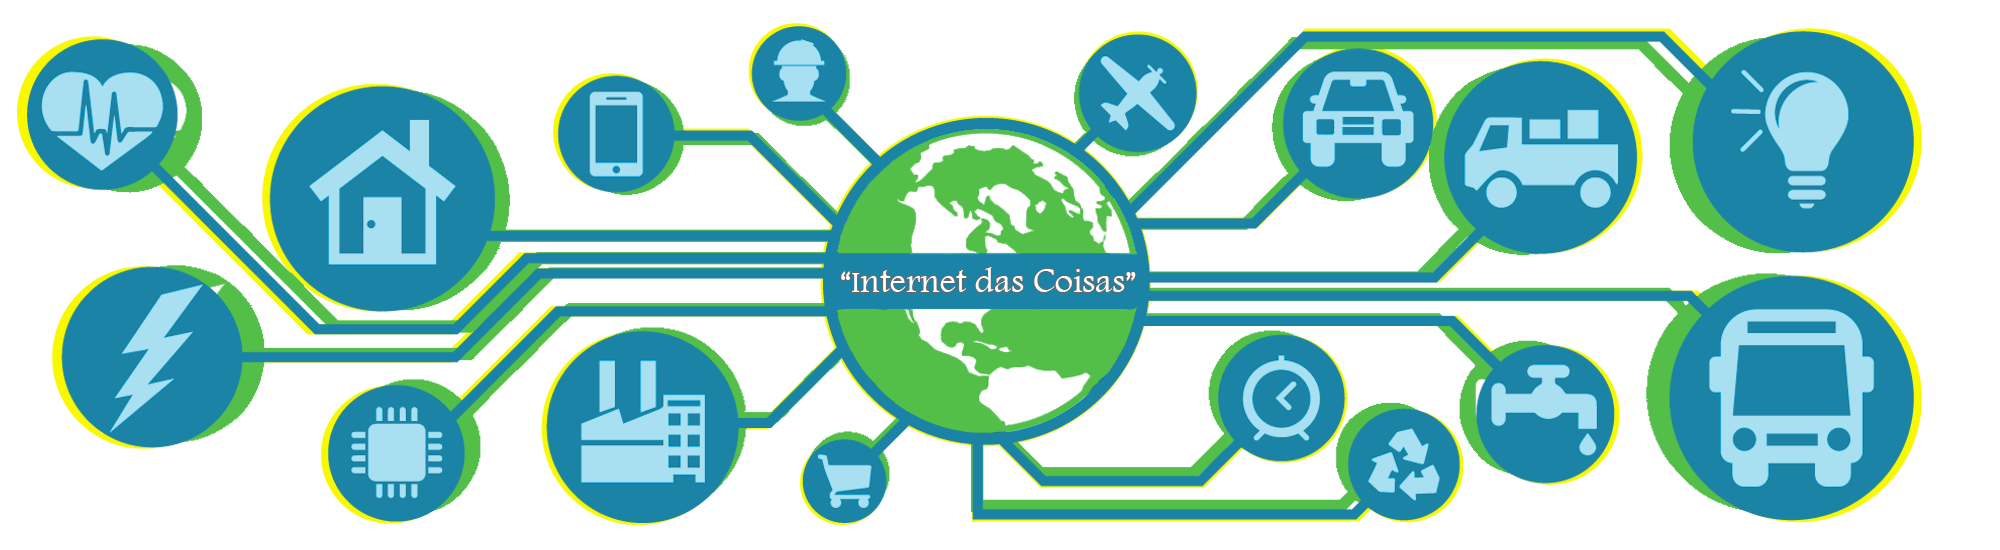
\includegraphics[scale=0.12]{figs/internet-coisas.png}
\caption{Legenda da figura}
\label{f.internet_coisas}
\end{figure}
\end{frame}

\subsection{Coluna Dupla com Figura}
\begin{frame}
\begin{columns}
\begin{column}{6cm}
\begin{figure}[h]
\caption{\small Legenda da figura.}
\centering
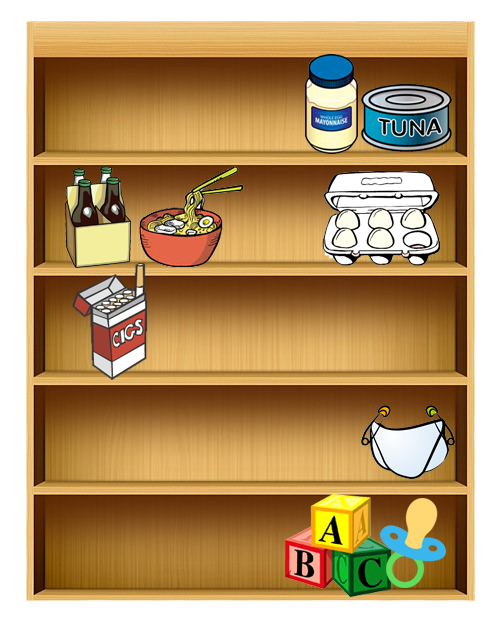
\includegraphics[scale=0.25]{figs/disposicao-mercado.png}
\label{f.disposicao_mercado}
\end{figure}
\end{column}
\begin{column}{5cm}
\begin{block}{\center \textbf{Exemplo}}
\justify Utilização de um bloco.
\end{block}
\end{column}
\end{columns}
\end{frame}

\subsection{Coluna Dupla}
\begin{frame}
\begin{columns}
\begin{column}{5cm}
\begin{itemize}
\item \justify Coluna Dupla;
\\~\\
\end{itemize}
\begin{itemize}
\item \justify Com 'itemize'.
\end{itemize}
\end{column}
\begin{column}{6cm}
\begin{block}{}
\center \textbf{\color{darkgreen}{Bloco de Cores}} x \alert{Diferentes}
\end{block}
\end{column}
\end{columns}
\end{frame}

\subsection{Citação}
\begin{frame}
\centering Utilizando citação~\cite{agrawal93}.
\begin{figure}[h]
\centering
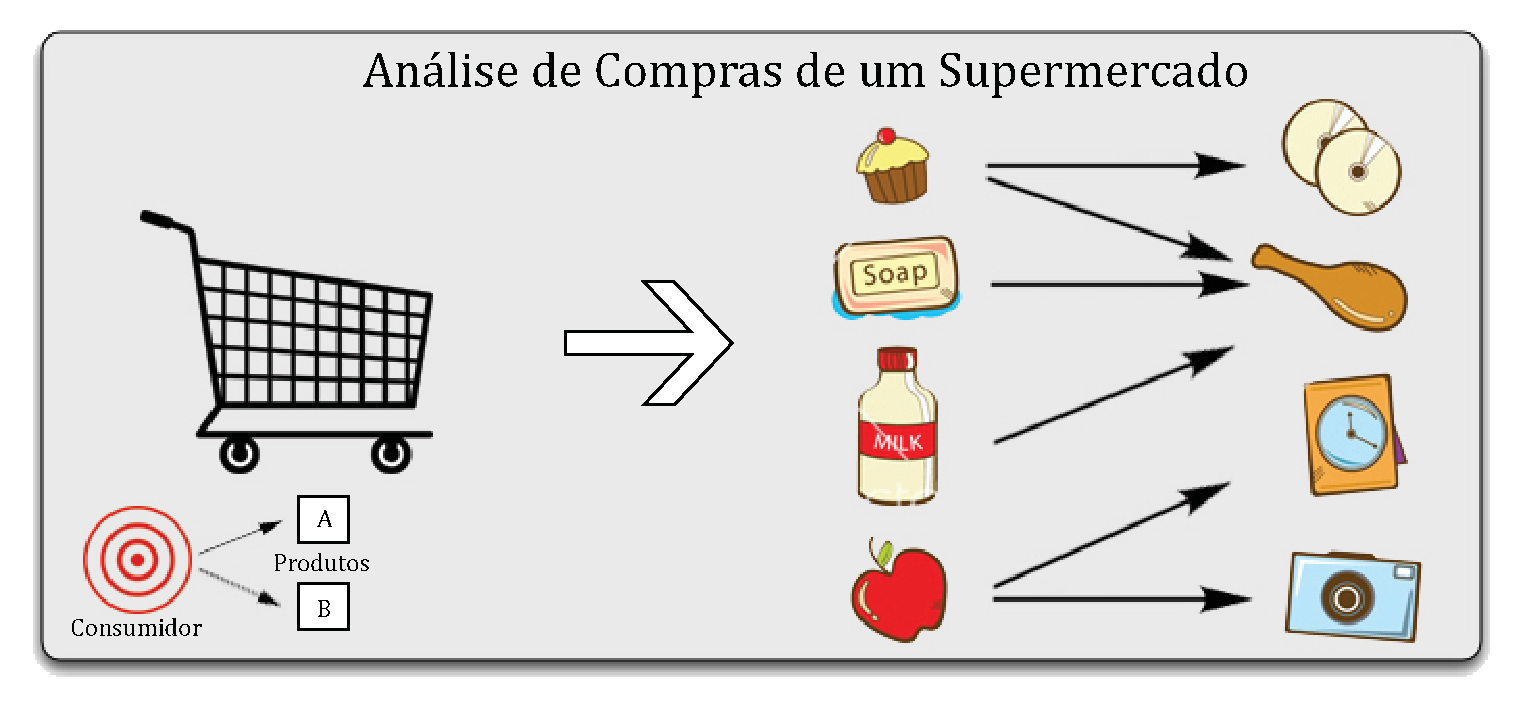
\includegraphics[scale=0.35]{figs/analise-mercado.pdf}
\caption{Legenda da figura.}
\label{f.analise_mercado}
\end{figure}
\end{frame}

\section{Seção 2}
\subsection{Utilizando Texto}
\begin{frame}\frametitle{Utilizando Texto}
\justify Texto normal.
\\~\\
\begin{itemize}
\item Item 1;
\item Item 2;
\item Item 3.	
\end{itemize}
\end{frame}

\subsection{Utilizando Tabelas}
\begin{frame}\frametitle{Utilizando Tabelas}
\begin{table}[h]
\centering
\begin{tabular}{c|c}
\hline
\textbf{\small TID} & \textbf{\small Conjunto de Itens}\\\hline \hline
{\small 1} & {\small \{Pão, Leite\}}\\\hline
{\small 2} & {\small \{Pão, Fralda, Cerveja, Ovos\}}\\\hline
{\small 3} & {\small \{Leite, Fralda, Cerveja, Coca-Cola\}}\\\hline
{\small 4} & {\small \{Pão, Leite, Fralda, Cerveja\}}\\\hline
{\small 5} & {\small \{Pão, Leite, Fralda, Coca-Cola\}}\\\hline
\end{tabular}
\caption{Legenda da tabela.}
\label{t.transacao_mercado}
\end{table}
\end{frame}

\section{Seção 3}
\subsection{Subseção}
\begin{frame}
\begin{block}{}
\justify \center Obrigado pela atenção!
\center \alert{Perguntas ou dúvidas?}
\end{block}
\begin{figure}[h]
\centering

\includegraphics[scale=0.15]{figs/questions.png}
\end{figure}	
\end{frame}

\end{document}